% THIS IS SIGPROC-SP.TEX - VERSION 3.0
% WORKS WITH V3.1SP OF ACM_PROC_ARTICLE-SP.CLS
% JUNE 2007
%
% It is an example file showing how to use the 'acm_proc_article-sp.cls' V3.1SP
% LaTeX2e document class file for Conference Proceedings submissions.
% ----------------------------------------------------------------------------------------------------------------
% This .tex file (and associated .cls V3.1SP) *DOES NOT* produce:
%       1) The Permission Statement
%       2) The Conference (location) Info information
%       3) The Copyright Line with ACM data
%       4) Page numbering
% ---------------------------------------------------------------------------------------------------------------
% It is an example which *does* use the .bib file (from which the .bbl file
% is produced).
% REMEMBER HOWEVER: After having produced the .bbl file,
% and prior to final submission,
% you need to 'insert'  your .bbl file into your source .tex file so as to provide
% ONE 'self-contained' source file.
%
% Questions regarding SIGS should be to
% Adrienne Griscti ---> griscti@acm.org
%
% Questions/suggestions regarding the guidelines, .tex and .cls files, etc. to
% Gerald Murray ---> murray@acm.org
%
% For tracking purposes - this is V3.0SP - JUNE 2007

\documentclass{sig-alternate}

\usepackage{times}
\usepackage{graphicx}
\usepackage{epsf}
\usepackage{verbatim}
\usepackage{psfig}
\usepackage{cite}
\usepackage{url}
\usepackage{color}
\usepackage{alltt}

\usepackage{longtable,lscape}
\usepackage{slashbox,multirow}
\usepackage{colortbl}
\usepackage{mathrsfs}

\newcommand{\Add}{\CodeIn{add}}
\newcommand{\AVTree}{\CodeIn{AVTree}}
\newcommand{\Assignment}[3]{$\langle$ \Object{#1}, \Object{#2}, \Object{#3} $\rangle$}
\newcommand{\BinaryTreeRemove}{\CodeIn{BinaryTree\_remove}}
\newcommand{\BinaryTree}{\CodeIn{BinaryTree}}
\newcommand{\Caption}{\caption}
\newcommand{\Char}[1]{`#1'}
\newcommand{\CheckRep}{\CodeIn{checkRep}}
\newcommand{\ClassC}{\CodeIn{C}}
\newcommand{\CodeIn}[1]{{\small\texttt{#1}}}
\newcommand{\CodeOutSize}{\scriptsize}
\newcommand{\Comment}[1]{}
\newcommand{\Ensures}{\CodeIn{ensures}}
\newcommand{\ExtractMax}{\CodeIn{extractMax}}
\newcommand{\FAL}{field-ordering}
\newcommand{\FALs}{field-orderings}
\newcommand{\Fact}{observation}
\newcommand{\Get}{\CodeIn{get}}
\newcommand{\HashSet}{\CodeIn{HashSet}}
\newcommand{\HeapArray}{\CodeIn{HeapArray}}
\newcommand{\Intro}[1]{\emph{#1}}
\newcommand{\Invariant}{\CodeIn{invariant}}
\newcommand{\JUC}{\CodeIn{java.\-util.\-Collections}}
\newcommand{\JUS}{\CodeIn{java.\-util.\-Set}}
\newcommand{\JUTM}{\CodeIn{java.\-util.\-TreeMap}}
\newcommand{\JUTS}{\CodeIn{java.\-util.\-TreeSet}}
\newcommand{\JUV}{\CodeIn{java.\-util.\-Vector}}
\newcommand{\JMLPlusJUnit}{JML+JUnit}
\newcommand{\Korat}{Korat}
\newcommand{\Left}{\CodeIn{left}}
\newcommand{\Lookup}{\CodeIn{lookup}}
\newcommand{\MethM}{\CodeIn{m}}
\newcommand{\Node}[1]{\CodeIn{N}$_#1$}
\newcommand{\Null}{\CodeIn{null}}
\newcommand{\Object}[1]{\CodeIn{o}\ensuremath{_#1}}
\newcommand{\PostM}{\MethM$_{post}$}
\newcommand{\PreM}{\MethM$_{pre}$}
\newcommand{\Put}{\CodeIn{put}}
\newcommand{\Remove}{\CodeIn{remove}}
\newcommand{\RepOk}{\CodeIn{repOk}}
\newcommand{\Requires}{\CodeIn{requires}}
\newcommand{\Reverse}{\CodeIn{reverse}}
\newcommand{\Right}{\CodeIn{right}}
\newcommand{\Root}{\CodeIn{root}}
\newcommand{\Set}{\CodeIn{set}}
\newcommand{\State}[1]{2^{#1}}
\newcommand{\TestEra}{TestEra}
\newcommand{\TreeMap}{\CodeIn{TreeMap}}

\newenvironment{CodeOut}{\begin{scriptsize}}{\end{scriptsize}}
\newenvironment{SmallOut}{\begin{small}}{\end{small}}

\newcommand{\pairwiseEquals}{PairwiseEquals}
\newcommand{\monitorEquals}{MonitorEquals}
%\newcommand{\monitorWField}{WholeStateW}
\newcommand{\traverseField}{WholeState}
\newcommand{\monitorSMSeq}{ModifyingSeq}
\newcommand{\monitorSeq}{WholeSeq}

\newcommand{\IntStack}{\CodeIn{IntStack}}
\newcommand{\UBStack}{\CodeIn{UBStack}}
\newcommand{\BSet}{\CodeIn{BSet}}
\newcommand{\BBag}{\CodeIn{BBag}}
\newcommand{\ShoppingCart}{\CodeIn{ShoppingCart}}
\newcommand{\BankAccount}{\CodeIn{BankAccount}}
\newcommand{\BinarySearchTree}{\CodeIn{BinarySearchTree}}
\newcommand{\LinkedList}{\CodeIn{LinkedList}}

\newcommand{\Book}{\CodeIn{Book}}
\newcommand{\Library}{\CodeIn{Library}}

\newcommand{\Jtest}{Jtest}
\newcommand{\JCrasher}{JCrasher}
\newcommand{\Daikon}{Daikon}
\newcommand{\JUnit}{JUnit}

\newcommand{\trie}{trie}

\newcommand{\Perl}{Perl}


\newcommand{\SubjectCount}{11}
\newcommand{\DSSubjectCount}{two}

\newcommand{\Equals}{\CodeIn{equals}}
\newcommand{\Pairwise}{PairwiseEquals}
\newcommand{\Subgraph}{MonitorEquals}
\newcommand{\Concrete}{WholeState}
\newcommand{\ModSeq}{ModifyingSeq}
\newcommand{\Seq}{WholeSeq}
\newcommand{\Aeq}{equality}

\newcommand{\Meaning}[1]{\ensuremath{[\![}#1\ensuremath{]\!]}}
\newcommand{\Pair}[2]{\ensuremath{\langle #1, #2 \rangle}}
\newcommand{\Triple}[3]{\ensuremath{\langle #1, #2, #3 \rangle}}
\newcommand{\SetSuch}[2]{\ensuremath{\{ #1 | #2 \}}}

\newcommand{\Equiv}[2]{\ensuremath{#1 \EquivSTRel{} #2}}
\newcommand{\EquivME}{\Equiv}
\newcommand{\EquivST}{\Equiv}
\newcommand{\EquivSTRel}{\ensuremath{\cong}}
\newcommand{\Redundant}[2]{\ensuremath{#1 \lhd #2}}
\newcommand{\VB}{\ensuremath{\mid}}
\newcommand{\MES}{method-entry state}

\newcommand{\Small}[1]{{\small{#1}}}

\newcommand{\CenterCell}[1]{\multicolumn{1}{c|}{#1}}


\begin{document}

\title{Automated Method Sequence Generation for Achieving Desirable Object States}
%
% You need the command \numberofauthors to handle the 'placement
% and alignment' of the authors beneath the title.
%
% For aesthetic reasons, we recommend 'three authors at a time'
% i.e. three 'name/affiliation blocks' be placed beneath the title.
%
% NOTE: You are NOT restricted in how many 'rows' of
% "name/affiliations" may appear. We just ask that you restrict
% the number of 'columns' to three.
%
% Because of the available 'opening page real-estate'
% we ask you to refrain from putting more than six authors
% (two rows with three columns) beneath the article title.
% More than six makes the first-page appear very cluttered indeed.
%
% Use the \alignauthor commands to handle the names
% and affiliations for an 'aesthetic maximum' of six authors.
% Add names, affiliations, addresses for
% the seventh etc. author(s) as the argument for the
% \additionalauthors command.
% These 'additional authors' will be output/set for you
% without further effort on your part as the last section in
% the body of your article BEFORE References or any Appendices.

%\numberofauthors{1} %  in this sample file, there are a *total*
% of EIGHT authors. SIX appear on the 'first-page' (for formatting
% reasons) and the remaining two appear in the \additionalauthors section.
%

%\author{Suresh Thummalapenta$^1$, Tao Xie$^1$, Nikolai Tillmann$^2$, Jonathan de Halleux$^2$, Wolfram Schulte$^2$\\
%\small{$^1$Department of Computer Science, North Carolina State University, Raleigh}\\
%\small{$^2$Microsoft Research, One Microsoft Way, Redmond}\\
%\small{$^1$\{sthumma, txie\}@ncsu.edu, $^2$\{nikolait, jhalleux, schulte\}@microsoft.com}\\
%}

%\author{
% You can go ahead and credit any number of authors here,
% e.g. one 'row of three' or two rows (consisting of one row of three
% and a second row of one, two or three).
%
% The command \alignauthor (no curly braces needed) should
% precede each author name, affiliation/snail-mail address and
% e-mail address. Additionally, tag each line of
% affiliation/address with \affaddr, and tag the
% e-mail address with \email.
%
% 1st. author
%\alignauthor
%Suresh Thummalapenta\\
%       \affaddr{Department of Computer Science}\\
%       \affaddr{North Carolina State University}\\
%       \affaddr{Raleigh, USA}\\
%       \email{sthumma@ncsu.edu}
%% 2nd. author
%\alignauthor
%Tao Xie\\
%			 \affaddr{Department of Computer Science}\\
%       \affaddr{North Carolina State University}\\
%       \affaddr{Raleigh, USA}\\
%       \email{xie@csc.ncsu.edu}% 3rd. author
%\and
%\alignauthor Nikolai Tillmann, Jonathan de Halleux, Wolfram Schulte\\
%       \affaddr{Microsoft Research}\\
%       \affaddr{One Microsoft Way, Redmond, USA}\\
%       \email{\{nikolait, jhalleux, schulte\}@microsoft.com}  
%}

\maketitle
%\begin{abstract}
%\end{abstract}

%\section{Introduction}
\label{sec:introduction}

Since the inception of computer science, many programming languages (\emph{e.g.}, Cobol, Fortran, or Java) have been introduced to serve specific requirements\footnote{\url{http://hopl.murdoch.edu.au}}. For example, Cobol is introduced specifically for developing business applications. In general, software companies or open source organizations often release their applications in different languages to survive in competing markets and to address various business requirements such as platform independence. An empirical study~\citep{jones1998estimating} shows that nearly one third applications have multiple versions in different languages. A natural way to implement an application in a different language is to translate from an existing application. For example, Lucene.Net was translated from Java Lucene according to its website\footnote{\url{http://lucene.apache.org/lucene.net/}}. As another example, the NeoDatis object database was also translated form Java to C\# according to its website\footnote{\url{http://wiki.neodatis.org/}}. During translation, one primary goal is to ensure that both applications exhibit the same behavior.

As existing applications typically use API libraries, it is essential to understand API mapping relations of one programming language, referred to as $L_1$, to another language, referred to as $L_2$, when translating applications from $L_1$ to $L_2$. Researchers~\citep{robillard2009makes,thomas2006api} pointed out that it is hard to use API elements, and our previous work~\citep{zhong2010mining} shows that mapping relations between API elements of different languages can also be complicated. In some cases, programmers may fail to find an existing API element that has the same behavior in the other language. For example, Figures~\ref{fig:db4ojava} and \ref{fig:db40net} show two methods implemented in db4o\footnote{\url{http://www.db4o.com}} of its Java version and its C\# version, respectively. When translating the Java code shown in Figure~\ref{fig:db4ojava} to C\#, programmers of db4o may fail to find an existing C\# class that has the same behaviors with the \CodeIn{Byte\-Array\-Input\-Stream} class in Java, so they implement a C\# class with the same name to fix the behavioral difference. Behavioral differences of mapped API elements (\emph{i.e}., classes, methods, and fields of API libraries) may occur in many places. To reduce translation effort, programmers of db4o developed their own translation tool, called Sharpen\footnote{\url{http://developer.db4o.com/Blogs/News/tabid/171/entryid/653/Default.aspx}}, for translating db4o from Java to C\#. For API translation, Sharpen systematically replaces all API elements in Java with equivalent elements in C\# to ensure that translated C\# applications have the same behaviors with the original Java ones.

\begin{figure}[t]
\begin{CodeOut}%\vspace*{-2ex}
\begin{alltt}
01: private long readLong(ByteArrayInputStream is)\{
02:  ...
03:  l += ((long) (is.read())) << i;
04:  ...\}
\end{alltt}
\end{CodeOut}%\vspace*{-4ex}
\caption{A method in the Java version of db4o.}%\vspace*{-2ex}
\label{fig:db4ojava}
\begin{CodeOut}%\vspace*{-2ex}
\begin{alltt}
05: private long ReadLong(ByteArrayInputStream @is)\{
06:  ...
07:  l += ((long)(@is.Read())) << i;
08:  ...\}
\end{alltt}
\end{CodeOut}%\vspace*{-4ex}
\caption{A method in the C\# version of db4o.}%\vspace*{-4ex}
\label{fig:db40net}
\end{figure}

In practice, as pointed out by Keyvan Nayyeri\footnote{\url{http://dotnet.dzone.com/print/26587}}, one of the most common problems is that translated code does not return expected outputs, partially because behavioral differences of mapped API elements are not fully fixed. For example, when JLCA\footnote{JLCA is a Java-to-C\# translation tool developed by Microsoft. The website of JLCA is \url{http://msdn.microsoft.com/en-us/magazine/cc163422.aspx}} translates the \CodeIn{java.lang.String.indexOf(int)} method from Java to C\#, it generates a warning message: ``Method \CodeIn{java.lang.String. indexOf} was converted to \CodeIn{System.String.IndexOf}, which may throw an exception''. Still, the report does not describe where such an exception is thrown or how to deal with that exception. As programmers typically do not know where such behavioral differences occur, it is difficult for programmers to fix such differences in advance, and thus defects can be introduced in translated applications. To prevent those defects, it is desirable to detect behavioral differences between mapped API elements in different languages. However, existing approaches~\citep{orso1using,jin2010automated,jiang2009automatic,lindigaadebug2005} solve different problems, and cannot detect such differences effectively since these existing approaches require that both the versions under consideration belong to the same language. In our context, the versions under consideration belong to different languages, making these existing approaches inapplicable.


To address the preceding issue, we propose a novel approach, called TeMAPI (\textbf{Te}sting \textbf{Ma}pping relations of \textbf{API}s), that generates test cases to detect behavioral differences among API mapping relations automatically. In particular, TeMAPI accepts two inputs: a translation tool under analysis and a test-generation tool for generating test cases. Given a translation tool that translates applications from one language $L_1$ to the other language $L_2$, TeMAPI generates various test cases to detect behavioral differences among the API mapping relations by effectively leveraging the test-generation tool. TeMAPI next executes translated test cases to detect behavioral differences.

TeMAPI addresses four major technical challenges in effectively detecting behavioral differences. (1) It is challenging to directly extract API mapping relations from translation tools. The primary reason is that often translation tools either use different formats for specifying API mapping relations or do not explicitly describe these mapping relations. For example, Java2CSharp\footnote{Java2CSharp is a Java-to-C\# translation tool developed by ILOG (now IBM). The website of Java2CSharp is \url{http://j2cstranslator.sourceforge.net/}} uses mapping files, Sharpen hardcodes relations in source files, and closed source translation tools such as JLCA typically hide mapping relations in binary files. To address this issue and to be independent of the translation tool under analysis, TeMAPI analyzes translated code for extracting those relations. (2) Interfaces of two mapped API elements can be different, and one API element can be translated to multiple API elements. For example, JLCA translates the \CodeIn{java.net.DatagramSocket.receive(DatagramPacket)} method in Java as shown in Figure~\ref{fig:javacode} to multiple C\# elements as shown in Figure~\ref{fig:codeJLCA}.
To address this issue, TeMAPI uses a technique, called wrapper methods (Section~\ref{sec:approach:wrapper}), that abstracts interface differences among mapped API elements and provides a common interface to effectively apply test-generation tools. (3) Using a basic technique such as generating test cases with \CodeIn{null} values may not be significant in detecting behavioral differences among API mapping relations. Since we focus on object-oriented languages such as Java or C\# to detect behavioral differences, generated test cases need to exercise various object states, which can be achieved using method-call sequences. To address this issue, TeMAPI leverages two existing state-of-the-art test-generation techniques: random~\citep{pacheco2007feedback} and dynamic-symbolic-execution-based~\citep{koushik:cute, godefroid:dart, tillmann2008pex} ones. (4) API elements are typically quite large in size, and it is difficult to check all outputs, posing a test oracle barrier. To overcome the barrier, TeMAPI uses return values of wrapper methods or exceptions being thrown as test oracles. We describe more details of our approach to address these challenges in subsequent sections.

In this paper, although we present our approach for detecting behavioral differences among mapping relations of different languages, our approach is general and can be applied to other software engineering problems where an API needs to be replaced with another API without changing the behavior of an application (\emph{e.g.}, library upgrades~\citep{Kawrykow:2009} or migrating from one library to another library~\citep{nita2010using}).

This paper makes the following major contributions:

\begin{itemize}\vspace*{-1ex}
\item A novel approach, called TeMAPI, that automatically generates test cases to detect behavioral differences among API mapping relations. %\vspace*{-1.5ex}
\item A tool implemented for TeMAPI and four evaluations on five popular translation tools. Unlike untranslated code elements, behavioral differences introduce no compilation errors to be detected, and can lead to defects in translated applications silently. Our results show that existing translation tools can translate most lines from Java to C\#, although these tools typically cover a small set of API mapping relations. Our results also show the effectiveness of our approach in detecting behavioral differences of mapped API elements between different languages.
\item The first empirical comparison on behavioral differences of mapped API elements between the J2SE and .NET frameworks. As shown in Section~\ref{sec:evaluation}, the comparison reveals 8 behavioral differences between mapped API elements in existing translation tools. We analyze these findings, and conclude their implications that are valuable to vendors of translation tools for improving their tools, programmers who use translation tools for being aware of such differences in advance, and developers of API libraries for implementing more translatable APIs.
\end{itemize}\vspace*{-1ex}

The rest of this paper is organized as follows.
%Section~\ref{sec:mapping} presents our test adequacy criteria.
Section~\ref{sec:example} presents an illustrative example.
Section~\ref{sec:approach} presents our approach.
Section~\ref{sec:evaluation} presents our evaluation.
Section~\ref{sec:real} presents capabilities of existing translation tools to translate real projects and discusses importance of our major findings.
Section~\ref{sec:discuss} discusses issues of our approach.
Section~\ref{sec:related} presents related work.
Section~\ref{sec:conclusion} concludes.
\begin{figure}[t]
\begin{CodeOut}%\vspace*{-2ex}
\begin{alltt}
09: DatagramSocket socket = ...;
10: DatagramPacket package = ...;
11: socket.receive(package);
\end{alltt}
\end{CodeOut}%\vspace*{-5ex}
\caption{Sample code in Java.}%\vspace*{-2ex}
\label{fig:javacode}
\begin{CodeOut}%\vspace*{-2ex}
\begin{alltt}
12: UdpClient socket = ...;
13: IPEndPoint remoteIpEndPoint = ...;
14: try\{
15:  byte[] data_in = socket.Receive(ref remoteIpEndPoint);
16:  PacketSupport tempPacket =
          new PacketSupport(data_in, data_in.Length);
17:   tempPacket.IPEndPoint = remoteIpEndPoint;
18: \} catch (System.Exception e)\{...\}
19: PacketSupport package = tempPacket;
\end{alltt}
\end{CodeOut}%\vspace*{-5ex}
\caption{Translated C\# code by JLCA.}%\vspace*{-4ex}
\label{fig:codeJLCA}
\end{figure}

%As stated by Sebesta~\citep{sebesta2002concepts}, modern programming languages start around 1958 to 1960 with the development of Algol, Cobol, Fortran and Lisp. Ever since then, thousands of programming languages came to existence as shown by HOPL website\footnote{\url{http://hopl.murdoch.edu.au}}. For various considerations, programmers often need to translate projects from one language to another language. For example, as stated by , to provide the language and platform independence, he translates Compose*~\citep{garcia-compose} in C\# to Compose*/J in Java. To relief the efforts of translating, programmers may use existing translation tools or even implement their own translation tools. For example, Salem \emph{et al.}~\citep{AgtashAEMBS06} report their experience of translating the BLUE financial system of the ICT company from Java to C\# by the JLCA\footnote{\url{http://tinyurl.com/2c4coln}} tool. For another example, to translate db4o\footnote{\url{http://www.db4o.com}} from Java to C\#, its programmers develop their own translation tool named Sharpen\footnote{\url{http://tinyurl.com/22rsnsk}}.

%To translate a source file, a translation tool needs to its structures and its used API elements. As a project typically use thousands of API elements, it is often more difficult to translate used API elements especially for those languages whose structures are similar. In particular, El-Ramly \emph{et al.}~\citep{el2006experiment} conduct an experiment to translate Java programs to C\#. One of their learnt lessons is ``it
%becomes very important to develop methods for
%automatic API transformation''. Barry compares C\# with Java\footnote{\url{http://tinyurl.com/26d8xcp}}, and claims ``although coding in C\# is easy for a Java programmer..., the biggest challenge in moving from Java to the .NET Framework is learning the details of another set of class libraries''. If not knowing API mapping relations, a translation tool or a programmer cannot translate used API elements correctly. Even when such mapping relations are available, a migration process may introduce defects in translated code since mapped API elements can have behavioral differences. As reported by Panesar\footnote{\url{http://tinyurl.com/3xpsdtx}}, even most common methods such as \CodeIn{String.subString(int, int)} can have behavioral differences between Java and C\#. We investigate the mapping relations of existing translation tools, and we confirm that the behavioral differences of mapped API elements can cause defects in translated code. In particular, in Java2CSharp\footnote{\url{http://j2cstranslator.sourceforge.net/}}, one item of mapping files is described in its mapping files as follows:
%
%\begin{CodeOut}%\vspace*{-2ex}
%\begin{alltt}
%1 package java.lang::System\{
%2  class java.lang.String :: System:String\{
%3   method valueOf(Object) { pattern = @1.ToString(); }
%4   ...\}\}
%\end{alltt}
%\end{CodeOut}
%
%Line 2 of this item describes that the \CodeIn{java.lang.String} class in Java is mapped to the \CodeIn{System.String} class in C\#. Line 3 of this item describes that the \CodeIn{java.lang.String.valueOf(Object)} method is mapped to the \CodeIn{System.String.ToString()} method in C\#, and \CodeIn{@1} denotes the first parameter of the \CodeIn{valueOf(Object)} method. Based on the preceding mapping relation, Java2CSharp translates a Java code snippet (Lines 5 and 6) to a C\# code snippet (Lines 7 and 8) as follows.
%
%\begin{CodeOut}%\vspace*{-2ex}
%\begin{alltt}
%\textbf{  Java Code}
%5 Object obj = ...
%6 String value = java.lang.String.valueOf(obj);
%\textbf{  C# Code translated by Java2CSharp}
%7 Object obj = ...
%8 String value = obj.ToString();
%\end{alltt}
%\end{CodeOut}
%
%The translated code snippet compile well, but it has behavioral differences with the original Java code snippet. For example, if Line 5 assigns null to \CodeIn{obj}, \CodeIn{value} of Line 6 will be ``null''. If Line 7 assigns null to \CodeIn{obj}, \CodeIn{value} of Line 8 will not be set to ``null'' since it throws \CodeIn{NullReferenceException}.
%
%As it throw exceptions, the preceding difference of API mapping relation is relatively easy to detect since programmers often use extreme inputs such as null values as test cases. In particular, Sharpen is aware of the differences, and the mapping relation in Sharpen is defined as follows:
%
%\begin{CodeOut}
%\begin{alltt}
%9 public abstract class Configuration \{
%10 protected void setUpStringMappings() \{
%11   mapMethod("java.lang.String.valueOf",
%              runtimeMethod("getStringValueOf"));
%12  ...\} \}
%\end{alltt}
%\end{CodeOut}
%
%Based on Line 11 of the preceding mapping relation, Sharpen translates the Java code snippet (Lines 5 and 6) to a C\# code snippet (Lines 7 and 8) as follows.
%
%\begin{CodeOut}%\vspace*{-2ex}
%\begin{alltt}
%\textbf{  C# Code translated by Sharpen}
%13 Object obj = ...
%14 String value = getStringValueOf(obj);
%\end{alltt}
%\end{CodeOut}
%
%In Sharpen, the \CodeIn{getStringValueOf(object)} method is implemented as follows:
%
%\begin{CodeOut}%\vspace*{-2ex}
%\begin{alltt}
%15 public static string GetStringValueOf(object value)\{
%16  return null == value? "null": value.ToString();
%17	\}
%\end{alltt}
%\end{CodeOut}
%
%If Line 13 assigns a null value to \CodeIn{obj}, \CodeIn{value} in Line 14 will also be ``null'' as expected. By implementing its own mapped C\# method, Sharpen hides the preceding difference, but it still fails to hide all differences. For example, we find that if Line 5 assigns a \CodeIn{false} boolean value to \CodeIn{obj}, \CodeIn{value} in Line 6 will be ``false'', but if Lines 7 and 13 assign a \CodeIn{false} boolean value to \CodeIn{obj}, \CodeIn{value} of Line 8 and \CodeIn{value} in Line 14 will both be ``False''. This difference is relatively difficult to detect, since a programmer typically does not know the internal logic of the method to construct appropriate test cases.
%
%
%It is desirable to detect differences of API mapping relations since the differences will potentially introduce defects to client codek, the same inputs, but it is challenging to detect behavioral differences of API mapping relations via testing for three factors: (1) API elements are typically quite large in size, so it takes great efforts to write test cases manually for API elements and their mapping relations; (2) Other types of migrations such as library migrations~\citep{nita2010using} can use existing test cases to ensure the quality of migrated code, but for language migration, translated test cases may also have defects at the first place; (3) It requires many test cases to reveal all behaviors of API elements, and simply generating extreme values such as null values are not sufficient to reveal all API behaviors.
%
%In this paper, we propose an approach, called TeMAPI (\textbf{Te}sting \textbf{Ma}pping relations of \textbf{API}s), that detects behavioral differences of API mapping relations via testing. TeMAPI generates various test cases and compares testing results of mapped API elements for their behavioral differences. This paper makes the following major contributions:
%
%\begin{itemize}\vspace*{-1.5ex}
%\item A novel approach, called TeMAPI, that detect behavioral differences of mapped API elements via testing. Given a translation tool, TeMAPI detects behavioral differences of its all API mapping relations automatically. It is important to detect these behavioral differences since they can introduce defects in translated code silently.\vspace*{-1.5ex}
%\item Test adequacy criteria proposed for generating sufficient test cases to test API mapping. TeMAPI targets at generating adequate test cases that can reveal all behaviors of API elements to test their mapping relations.\vspace*{-1.5ex}
%\item A tool implemented for TeMAPI and two
%evaluations on ?? projects that include ?? mapping relations from Java to C\#, and ?? mapping relations from C\# to Java. The results show that our tool detects ?? unique defects of mapping relations...
%\end{itemize}\vspace*{-1.5ex}
%
%The rest of this paper is organized as follows.
%Section~\ref{sec:mapping} presents our test adequacy criteria.
%Section~\ref{sec:example} illustrates our approach using an example.
%Section~\ref{sec:approach} presents our approach.
%Section~\ref{sec:evaluation} presents our evaluation results.
%Section~\ref{sec:discuss} discusses issues of our approach.
%Section~\ref{sec:related} presents related work.
%Finally, Section~\ref{sec:conclusion} concludes.

%\section{Example}
\label{sec:example}

TeMAPI includes three major steps in detecting behavioral differences among API elements described in mapping relations. We use JLCA (a Java-to-C\# translation tool) as an example translation tool, and the \CodeIn{java.io.ByteArrayInputStream} class in Java as an example API element to illustrate these three steps.

%----------------------------------------------------
\textbf{Translating Synthesized wrappers.} TeMAPI first synthesizes a Java wrapper class for the example class. TeMAPI next uses JLCA to translate the wrapper class to C\#. TeMAPI compares source code of the synthesized wrapper class with the translated wrapper class to extract translatable API elements of the example class. In particular, our example class in Java has five fields, two constructors, and eight methods besides inherited ones\footnote{\url{http://tinyurl.com/2dsgftv}}. A class can have more than one constructor, and a translation tool may not translate all its constructors. Therefore, to address this issue, TeMAPI includes different constructors in its synthesized wrapper methods instead of simply pushing the receiver object as a parameter of wrapper methods. For example, TeMAPI first identifies \CodeIn{ByteArrayInputStream(byte[])} constructor as translatable, and synthesizes the wrapper method for the \CodeIn{skip(long)} method as follows:

\begin{CodeOut}\vspace*{-1ex}
\begin{alltt}
public long testskip24nm(long m0, byte c0[])\{
  ByteArrayInputStream obj = new ByteArrayInputStream(c0);
  return obj.skip(m0);\}
\end{alltt}
\end{CodeOut}\vspace*{-2ex}

TeMAPI next uses JLCA to translate synthesized wrapper methods from Java to C\#. A translation tool typically cannot include mapping relations for all the API elements between two languages, so translated wrapper methods can have compilation errors. TeMAPI parses translated wrapper methods and filters out all methods with compilation errors. For example, below is the translated \CodeIn{testskip- 24nm} method in C\#:
\vspace*{-2ex}

\begin{CodeOut}
\begin{alltt}
public virtual long testskip24nm(long m0, sbyte[] c0)\{
  MemoryStream obj = new MemoryStream(
                    SupportClass.ToByteArray(c0));
  MemoryStream temp_BufferedStream = obj;
  Int64 temp_Int64 = temp_BufferedStream.Position;
  temp_Int64 = temp_BufferedStream.Seek(m0,
       System.IO.SeekOrigin.Current) - temp_Int64;
  return temp_Int64;\}
\end{alltt}
\end{CodeOut}\vspace*{-2ex}

TeMAPI does not remove this method, since it does not result in compilation errors.


\textbf{Generation of C\# Test Cases for Testing Java Code.} A major advantage of our synthesized wrapper is that the original wrapper and the translated wrapper shares the same interface, irrespective of method calls within the wrapper method. Therefore, TeMAPI detects behavioral differences between mapped API elements by generating test cases on one version of wrapper methods and applying those test cases on the other version. In particular, TeMAPI extends Pex~\cite{tillmann2008pex} to generate test cases for each remaining C\# wrapper method. For the example class, Pex attempts to explore all feasible paths among method calls within the wrapper methods and generates inputs and outputs that exercise various paths. Based on the inputs and output generated for each path, TeMAPI generates a Java test case to check whether the original wrapper method return the same values as the translated one. For example, TeMAPI generates the following Java test case based on inputs generated by Pex for one feasible path (in the C\# wrapper method) that throws exceptions.

\begin{CodeOut}\vspace*{-1ex}
\begin{alltt}
public void testskip24nm36()\{
  try\{
     Test_java_io_ByteArrayInputStream obj =
        new Test_java_io_ByteArrayInputStream();
     long m0 = java.lang.Long.valueOf(
                  "2147483648").longValue();
     byte[] c0 = new byte[0];
     obj.testskip24nm(m0,c0);
     Assert.assertTrue(false);
  \}catch(java.lang.Exception e)\{
     Assert.assertTrue(true); \}\}
\end{alltt}
\end{CodeOut}\vspace*{-2ex}

This Java test case fails, since given the preceding inputs, the \CodeIn{skip (long)} method in Java does not throw any exceptions, instead the translated C\# code does. Thus, TeMAPI detects a behavioral difference between the \CodeIn{skip(long)} method in Java and its translated C\# API elements by JLCA.

%-----------------------------------
\textbf{Generation of Java Test Cases for Testing C\# Code.} As shown by Thummalapenta \emph{et al.}~\cite{thummalapenta09:mseqgen}, Pex cannot effectively generate sequences. To address this issue, TeMAPI extends Randoop~\cite{pacheco2007feedback} for testing Java code to generate invocation sequences. TeMAPI does not generate invocation sequences from wrappers directly, since each wrapper method includes a fixed simple invocation sequence. Instead, TeMAPI uses translatable API methods in Step 1, and limits the scope of Randoop to those methods while generating invocation sequences. For example, a generated Java test case is as follows:

\begin{CodeOut}\vspace*{-1ex}
\begin{alltt}
public void test413() throws Throwable\{
  ...
  ByteArrayInputStream var2=new ByteArrayInputStream(...);
  var2.close();
  int var5=var2.available();
  assertTrue(var5 == 1);\}
\end{alltt}
\end{CodeOut}\vspace*{-2ex}


The test case gets passed, since Java allows access to the stream even if the stream is closed. TeMAPI next uses JLCA to translate the generated Java test case from Java to C\#. Since the Java test case uses only translatable API elements, JLCA translates the test case to a C\# test case as follows:

\begin{CodeOut}\vspace*{-1ex}
\begin{alltt}
public void test413() throws Throwable\{
  ...
  MemoryStream var2 = new MemoryStream(...);
  var2.close();
  long available = var2.Length - var2.Position;
  int var5 = (int) available;
  AssertTrue(var5 == 1);\}
\end{alltt}
\end{CodeOut}\vspace*{-2ex}

In contrast to the Java test case, the C\# test case gets failed since C\# does not allow such access to the stream and throws \CodeIn{ObjectDis\\posedException}. TeMAPI thus detects a behavioral difference with invocation sequences.

This example motivates our basic idea of generating test cases in one language and translating those test cases to another language for detecting differences among API mapping relations. %We next present details of our approach.

%\begin{figure}[t]
%\centering %\hfill
%\includegraphics[scale=0.95,clip]{figure/sample.eps}\vspace*{-3ex}
% \caption{\label{fig:example}API mapping}\vspace*{-4ex}
%\end{figure}

%Based on the mapping relations, a translation tool can migrate the
%preceding code snippet automatically. To learn the mapping
%relations,
%
%%\begin{figure}[t]
%%\centering
%%\includegraphics[scale=0.86,clip]{figure/openfile.eps}\vspace*{-1.5ex}
%% \caption
%%{\label{fig:openfile}Aligned wrapper}\vspace*{-2ex}
%%\end{figure}
%
%In this section, we illustrate the main steps of MAM to
%mine the API mapping in Java for \CodeIn{System.IO.Directory.
%Exists()} in C\# from the HypoLog
%project\footnote{\url{http://sourceforge.net/projects/twlog/}}.
%
%The first step of MAM is to align classes and methods of
%wrapper by names. This step finds class pairs and method pairs
%that implement similar functionalities, and each pair may use
%API mapping since it implements a similar functionality. Our
%approach chooses names to align classes and methods because these
%classes and methods are from the same project. In this example, our
%approach aligns the two methods as shown in
%Figure~\ref{fig:openfile} because the two method have similar names
%and their declaring classes also have similar names (see
%Section~\ref{sec:approach:alignclientcode} for details).
%
%The second step of MAM is to mine mapping relations of API
%classes based on the names of corresponding fields, parameters,
%returned types, and local variables. This step also relies on names
%for the same consideration of the first step. For example, our
%approach maps the two parameters with the same name as shown by the
%red arrow of Figure~\ref{fig:openfile}. From the types of the two
%parameters, MAM mines the mapping relation between two API
%classes: \CodeIn{System.String} $\leftrightarrow$
%\CodeIn{java.lang.String} (see
%Section~\ref{sec:approach:mappingtypes} for details).
%
%
%The final step of MAM is to mine mapping relations of API
%methods. Besides the factors listed in
%Section~\ref{sec:introduction}, another factor is that API calls in
%wrapper are often not carefully aligned. To deal with those
%challenges, MAM first builds an API Transformation Graph
%(ATG) for each method. After that, MAM compares built
%graphs to mine mapping relations of API methods (see
%Section~\ref{sec:approach:mappingtypes} and
%Figure~\ref{fig:approach1} for details). Figure~\ref{fig:example}
%shows the mined mapping relation between
%\CodeIn{System.IO.Directory.Exists()} and its API mapping in
%Java.

%\section{Approach}
\label{sec:approach}

Our approach accepts a set of projects as data sources and mines
API mapping between two different languages $L_1$ and $L_2$.
As mined API mapping describes mapping relations of APIs between
the two languages, this mapping is useful for language migration between the two languages.
For each project used as a data source, our approach requires
atleast two versions of the project (one version in $L_1$ and
the other version in $L_2$). Figure~\ref{fig:approach} shows
the overview of our approach.

First, our approach aligns client code in languages $L_1$ and $L_2$
so that the aligned source files implement similar functionalities
(Section~\ref{sec:approach:acc}). Second, our approach mines
mapping relations of API classes (Section~\ref{sec:approach:mappingtypes}).
Finally, our approach mines mapping relations of API
methods (Section~\ref{sec:approach:mappingtypes}) defined by the mapped
API classes.

\begin{figure}[t]
\centering
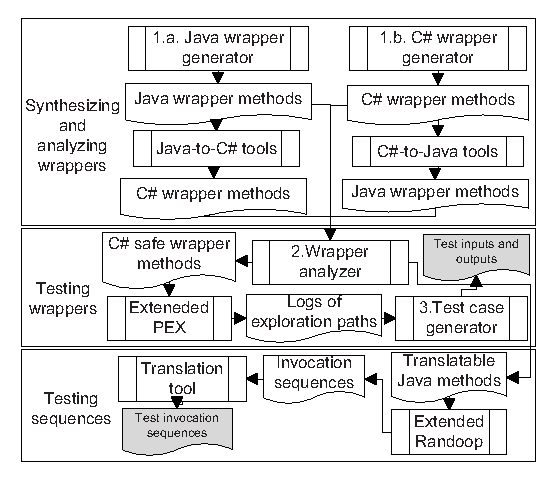
\includegraphics[scale=1,clip]{figure/approach.eps}\vspace*{-3ex}
 \caption{Overview of our approach}\vspace*{-3.5ex}
 \label{fig:approach}
\end{figure}

%-------------------------------------------------------------------
\subsection{Aligning Client Code}
\label{sec:approach:acc}

Initially, our approach accepts two versions of a project (one version in
$L_1$ and the other version in $L_2$) and aligns classes and methods
of the two versions. Aligned classes or methods
between the two versions implement a similar functionality. As they
implement a similar functionality, APIs used by these classes or methods can be
replaceable.

To align classes and methods of the two versions, our approach uses
name similarities between entities (such as class names or method names)
defined by the two versions of the project. In our approach, we have two
different kinds of entity names: entity names defined by the two versions
of the project and entity names of third-party libraries used by the two versions of the project.
The first kind often comes from the same programmer or the same team, or
programmers may refer to existing versions for naming entities such
as classes, methods, and variables. Therefore, name similarity is often
reliable to distinguish functionalities of the first kind compared to the second
kind. Our approach uses Simmetrics\footnote{\url{http://sourceforge.net/projects/simmetrics/}}
to calculate name similarities.

Algorithm 1 shows how our approach aligns client code classes. The
first step is to find candidate class pairs by names. For two sets
of classes ($C$ and $C'$), the algorithm returns candidate class
pairs ($M$) with a similarity greater than a given threshold,
referred to as \emph{SIM\_THRESHOLD}. As some projects may have many
classes with the same name, $M$ may contain more than one matching
pair for a class in a version. To align those classes, our algorithm
uses package names of these classes to refine $M$ and returns only
one matching pair with the maximum similarity\footnote{For C\#, we
refer to namespace names for package names.}.

In each aligned class pair, our approach further aligns methods
within the class pair. The algorithm for methods is similar to the
algorithm for classes but relies on other criteria such as the number of parameters
and names of parameters to refine candidate method pairs. These candidates
may contain more than one method pair due to overloading.
For the example shown in Section~\ref{sec:example}, our approach
correctly aligns the class \CodeIn{IndexFiles} and the method
\CodeIn{main} in Java to the class \CodeIn{IndexFiles}
and the method \CodeIn{Main} in C\# as their names are quite
similar.
%-----------------------------------------------------------------
\subsection{Mapping API classes}
\label{sec:approach:mappingtypes}

In this step, our approach mines mapping relations of
API classes. As defined in Section~\ref{sec:mapping}, mapping relations of API classes are used
to translate variables. Consequently, our approach mines mapping
relations of API classes based on how aligned client code declares
variables such as fields of aligned classes, parameters of aligned methods
and local variables of aligned methods. In
particular, for each aligned class pair $\Pair{c_1} {c_2}$, our
approach analyzes each field pair $\Pair{f_1}{f_2}$ and considers
$\Pair{f_1.type} {f_2.type}$ as one mined mapping relation of API
classes when the similarity between $f_1.name$ and $f_2.name$ is
greater than \emph{SIM\_THRESHOLD}. Similarly, for each aligned method pair
$\Pair{m_1} {m_2}$, our approach analyzes each local variable pair
$\Pair{var_1} {var_2}$ and considers $\langle var_1.type,$ $
var_2.type\rangle$ as one mined mapping relation of API classes when
the similarity between $var_1.name$ and $var_2.name$ is greater than
a threshold. Also, our approach analyzes each parameter pair
$\langle para_1, $ $para_2\rangle$ of $m_1$ and $m_2$, and our
approach considers $\langle para_1.type,$ $para_2.type\rangle$ as
one mined mapping relation of API classes when the similarity
between $para_1.name$ and $para_2.name$ is greater than \emph{SIM\_THRESHOLD}.

For the example shown in Section~\ref{sec:example}, our approach
mines the mapping relation between \CodeIn{java.io.File} and
\CodeIn{System.IO.FileInfo} based on the matched fields of Lines 4
and 9 (Figure~\ref{fig:clientcode}). The mapping relation of API classes helps translate the
variable declared in Line 1 (Figure~\ref{fig:totranslation})
to the variable declared in Line 16 (Figure~\ref{fig:translatedcode}).

%\begin{algorithm}[t]
%\begin{SmallOut}
%\dontprintsemicolon
%  \KwIn{$C$ is the classes of a language; $C'$ is the classes
%  of another language}
%  \KwOut{$P$ is aligned pairs of classes}
%  \Begin{
%     $M \leftarrow findCandidateClassPairs(C, C')$\;
%     \While{$M.size > 0 $}{
%        \If{$M.size > 1$}{
%            $M \leftarrow refineByPackageNames(M)$\;
%         }
%         \If{$M.size == 1$}{
%                $P.add(M)$\;
%                $C.remove(M[0].c)$\;
%                $C'.remove(M[0].c')$\;
%         }
%         $M \leftarrow findCandidateClassPairs(C, C')$\;
%     }
% }
%\end{SmallOut}
%\label{alg:alignclasses} \caption{Align Classes Algorithm}
%\end{algorithm}

\begin{figure}[t]
\centering
\includegraphics[scale=1,clip]{figure/algorithm1.eps}
\vspace*{-6ex}
\end{figure}

%-----------------------------------------------------------
\subsection{Mapping API methods}
\label{sec:approach:mappingtypes}

In this step, our approach mines mapping relations of API methods.
This step has two major sub-steps. First, our approach builds a graph, referred
as API transformation graph, for each client code
method. Second, our approach compares the two graphs of each paired
client code methods for mining mapping relations of API methods.

\begin{figure*}[t]
\centering
\includegraphics[scale=1.1,clip]{figure/graph.eps}\vspace*{-3ex}
 \caption
{\label{fig:graph}Built ATGs and the main steps of comparing
ATGs}\vspace*{-3.5ex}
\end{figure*}


\subsubsection{API transformation graph}
We propose API transformation graphs (ATG) to help deal with the two
challenges of mining API mapping listed in
Section~\ref{sec:introduction}. An API transformation graph of a
client code method $m$ is a directed graph
$G\Triple{N_{data}}{N_{m}}{E}$. $N_{data}$ is a set of the fields
$F$ of $m$'s declaring class, local variables $V$ of $m$, parameters
$P_1$ of $m$, parameters $P_2$ of methods called by $m$, and return
values $R$ of all methods. $N_{m}$ is a set of methods called by
$m$. $E$ is a set of directed edges. An edge $d_1\rightarrow d_2$
from a datum $d_1 \in N_{data}$ to a datum $d_2 \in N_{data}$
denotes the data dependency from $d_1$ to $d_2$. An edge $d_1
\rightarrow m_1$ from a datum $d_1 \in N_{data}$  to a method $ m_1
\in N_{m}$ denotes $d_1$ is a parameter or a related variable of
$m_1$. An edge $m_1 \rightarrow d_1$ from a method $m_1 \in N_{m}$
to a datum $d_1 \in N_{data}$ denotes $d_1$ is the return value of
$m_1$.

%We propose ATG for two main purposes. The first purpose is to mine mapping
%relations among parameters of mapped API methods. Mining mapping relations
%among parameters of mapped API methods is challenging as often mapped API methods
%can have different number of parameters or different positions among
%parameters. For example, consider the following two mapped API methods:
%
%\begin{CodeOut}
%$m_1$ in Java: BigDecimal java.math.BigDecimal.multiply (BigDecimal $p_1^1$)\\
%\hspace*{0.11in}$m_2$ in C\#: Decimal System.Decimal.Multiply (Decimal $p_1^2$, Decimal $p_2^2$)
%\end{CodeOut}
%
%Method $m_1$ of Java has a receiver variable, say $v_1^1$, of type \CodeIn{BigDecimal}
%and has one parameter $p_1^1$. The mapped method $m_2$ in C\# has
%two parameters $p_1^2$ and $p_2^2$. Using ATGs, our approach
%identifies that $v_1^1$ is mapped to $p_1^2$ and $p_1^1$ is mapped
%to $p_2^2$. As ATG captures parameters of API methods,
%our approach is able to deal with the challenges of mapping parameters.
%
%The second purpose of ATG is to mine mapping relations of merged API methods. As ATG
%describes data dependencies among inputs and outputs, our approach
%is able to mine mapping relations for merged API methods as shown in
%Figure~\ref{fig:example}. We next describe how our approach builds ATGs and
%uses ATGs for mining mapping relations of API methods.

\subsubsection{Building API transformation graphs }

Our approach builds an ATG for each method $m$. ATG includes information such as
inputs and outputs for each client code method. In particular, for
each method $m$, our approach first builds subgraph for its variables,
API methods, and field accesses according to the following rules:

%First, programming languages typically provide a huge set of APIs,
%and it is difficult to build mapping relations for all APIs
%manually. Second, some API methods have multiple parameters, and
%some parameters cannot be mapped directly one by one in orders. For
%example, \CodeIn{org.w3c.dom.Element.getAttributeNS()} and
%\CodeIn{System.Xml.XmlElement.GetAttribute()} both have two
%parameters, but the two parameters are inverse by their meanings.
%Third, one API method in one language may be mapped to more than one
%API method in other languages. For example, \CodeIn{java.util.
%LinkedList.removeLast()} returns the last value, and \CodeIn{System.
%Collections.Generic.LinkedList.RemoveLast()} does not return any
%values. To get that value, C\# programmers need to call more APIs,
%and thus one API method of Java is mapped to serval API methods of
%C\#.



%
%One challenge to mine mapping relations of two API methods lies in
%how to map their inputs correctly. Here, our approach both the
%receiver and the parameters of a method as the inputs of a
%method. Inputs of two API methods may be matched but are not in the
%same order. For example, as shown in Section~\ref{sec:example},
%\CodeIn{java.io. File.exist()} has a receiver whereas
%\CodeIn{System.IO.File.Exist()} has no receiver but a
%parameter. In addition, parameter orders may be quite different. For
%example, the parameter order of \CodeIn{org.w3c.
%dom.Element.getAttributeNS()} is inverse with the parameter order of
%\CodeIn{System.Xml.XmlElement.GetAttribute()}. To deal with the
%preceding problem,


\begin{enumerate}\vspace*{-2ex}
\item $\forall$ $f \in F \cup V \cup P_1$, our approach adds a node to the built ATG.
The reason for considering these variables such as fields in
declaring class or local variables in method $m$ used in client code
is that these variables are useful to analyze data dependencies
among API methods.\vspace*{-2ex}
%\begin{center}
%\includegraphics[scale=0.7,clip]{figure/rule1.eps}
%\end{center}
\item $\forall$ API methods of the form ``$T_0\ T.AM (T_1 p_1, \ldots, T_n p_n)$''
called by method $m$, our approach adds receiver (of type $T$) and
parameter nodes to the built ATG as shown below. Our approach does
not add receiver node for static API methods. \vspace*{-3ex}
\begin{center}
\includegraphics[scale=0.7,clip]{figure/rule2.eps}%\vspace*{-1.5ex}
\end{center}\vspace*{-3ex}
\item $\forall$ $f\in F \cup V$, if $f$ is a non-primitive variable
of type $T_1$ and a field $x$ of $T_1$ is accessed as $f.x$, our
approach adds nodes to the built ATG as shown below. As Java often
uses getters and setters whereas C\# often use field accesses, our
approach treats field accesses as a special type of method
calls.\vspace*{-2ex}
\begin{center}
\includegraphics[scale=0.7,clip]{figure/rule3.eps}%\vspace*{-1.5ex}
\end{center}\vspace*{-3ex}
\end{enumerate}

Our approach adds additional edges to the built ATG (and sub-graphs
inside ATG) representing data dependencies among built sub-graphs.
We use the following rules for adding additional edges to the built
ATG. \Comment{In particular, our approach analyzes source files of a
client code method statement by statement and adds edges according
to the rules as follows:} \vspace*{-1.5ex}
\begin{enumerate}
\item $\forall$ statements of the form $x = y$, where $x \in F \cup V \wedge y \in F \cup V$,
our approach adds an edge from $y$ to $x$. This edge represents that
$x$ is data dependent on $y$.\vspace*{-1.5ex}
\begin{center}
\includegraphics[scale=0.7,clip]{figure/rule4.eps}%\vspace*{-1.5ex}
\end{center}\vspace*{-1.5ex}
\item $\forall$ statements of the form $x = AM()$, where $x \in F \cup V$, our approach
adds an edge from $AM$ to $x$ if the return value of $AM$ is
assigned to $x$. This edge represents that $x$ is data dependent on
the return value of $AM$. \vspace*{-1.5ex}
\begin{center}
\includegraphics[scale=0.7,clip]{figure/rule5.eps}%\vspace*{-1.5ex}
\end{center}\vspace*{-1.5ex}
\item $\forall$ API methods $AM(x)$ called by method $m$, our approach
adds an edge from $x$ to the parameter node of $AM$. This edge
represents that the parameter of $AM$ is data dependent on
$x$.\vspace*{-1.5ex}
\begin{center}
\includegraphics[scale=0.7,clip]{figure/rule6.eps}%\vspace*{-1.5ex}
\end{center}\vspace*{-1.5ex}
\item $\forall$ statements of the form $m_2(m_1(x))$, our approach
adds an edge from the return value node of $m_1$ to the parameter
node of $m_2$ parameter node. This edge represents that the
parameter of $m_2$ is data dependent on the return value of
$m_1$.\vspace*{-1.5ex}
\begin{center}
\includegraphics[scale=0.7,clip]{figure/rule7.eps}%\vspace*{-1.5ex}
\end{center}\vspace*{-1.5ex}
\item $\forall$ statements of the form $x.m()$, our approach adds
an edge from $x$ to $m$ as $x$ is the receiver object of $m$. This
edge represents that the receiver object of $m$ is data dependent on
$x$.\vspace*{-1.5ex}
\begin{center}
\includegraphics[scale=0.7,clip]{figure/rule8.eps}%\vspace*{-1.5ex}
\end{center}\vspace*{-1.5ex}
\item $\forall$ statements of the form $ x = y\ op\ z\ op\ \ldots, op \in \{+,-,*,/\}$,
our approach adds edges from $y$, $z$, and others to $x$, as these
variables are connected by binary operations and the return value is
assigned to $x$. The edge denotes the data dependency from $y$, $z$,
and other variables to $x$. For simplicity, our approach ignores
\emph{op} info. We discuss the issue in
Section~\ref{sec:discuss}.\vspace*{-1.5ex}
\begin{center}
\includegraphics[scale=0.7,clip]{figure/rule9.eps}%\vspace*{-1.5ex}
\end{center}\vspace*{-2ex}
\end{enumerate}

For each method $m$ in the client code, our approach applies preceding
rules for each statement from the beginning to the end of $m$.
Within each statement, our approach applies these rules based on
their nesting depth in the abstract syntax tree. For example,
for the statements of the form $m_2(m_1(x))$, our approach first applies
these rules on $m_1$ and then on $m_2$.

Figures~\ref{fig:graph}a and ~\ref{fig:graph}b show partial ATGs for
C\# (\CodeIn{IndexFiles.cs}) and Java (\CodeIn{IndexFiles.java})
code examples shown in Figure~\ref{fig:clientcode}, respectively.
Figure~\ref{fig:graph} also shows corresponding line numbers of each
sub-graph. Our approach applies Rules 2 and 6 for Lines 4 and 9 (Figure~\ref{fig:clientcode})
to build corresponding sub-graphs in the ATG. For
Lines 6 and 7 (Figure~\ref{fig:clientcode}), our approach applies Rules 2 and 8 to build
corresponding sub-graphs in the ATG. For Lines 12 and 15 (Figure~\ref{fig:clientcode}),
our approach applies Rule 2, 3, and 6 to build corresponding sub-graphs.

%\begin{algorithm}[t]
%\begin{SmallOut}
%\label{alg:mapATG} \dontprintsemicolon
%  \KwIn{$G$ is the ATG of a method ($m$); $G'$ is the ATG of $m$'s mapped method.}
%  \KwOut{$S$ is a set of mapping relations for API methods}
%  \Begin{
%     $P \leftarrow findVarPairs(m, m')$\;
%     \For{Pair p in P}{
%        $SM \leftarrow G.nextMethods(p.sharp)$\;
%        $JM \leftarrow G.nextMethods(p.java)$\;
%        $\Delta S = mapping(SM, JM)$\;
%        \While{$\Delta S \neq \phi| \Delta SM \neq \phi| \Delta JM \neq \phi$}{
%            $S.addAll(\Delta S)$\;
%             \For{Method sm in SM}{
%                 \If{$sm.isMapped$}{
%                    $SM.replace(sm, sm.nextMethod())$\;
%                  }\Else{
%                    $SM.replace(sm, sm.mergeNextMethod())$\;
%                  }
%             }
%             \For{Method jm in JM}{
%                 \If{$jm.isMapped$}{
%                    $JM.replace(jm, jm.nextMethod())$\;
%                  }\Else{
%                    $JM.replace(jm, Jm.mergeNextMethod())$\;
%                  }
%             }
%             $\Delta S = mapping(SM, JM)$\;
%        }
%     }
% }
% \end{SmallOut}
%\caption{ATG Comparison Algorithm}
%\end{algorithm}

\begin{figure}[t]
\centering
\includegraphics[scale=1,clip]{figure/algorithm2.eps}
\vspace*{-6ex}
\end{figure}

%--------------------------------------------------------------------
\subsubsection{Comparing API transformation graphs}

The second sub-step compares each pair of built ATGs for mining mapping
relations of API methods. Our mapped API methods satisfy three
criteria: (1) Mapped API methods implement the same
functionality. (2) Mapping relation describes the relation
between parameters of mapped API methods. (3) Mapping relation
describes the relation between return values of
mapped API methods. The two mapped API methods in two
different languages satisfying the preceding three criteria
are replaceable in the client code. Therefore, these mapped API
methods assist for migrating client code from one language to another.

Algorithm 2 presents major steps of comparing ATGs for mining
mapping relations of API methods. Consider two methods $m$ and $m'$
of two different languages $L$ and $L'$, respectively, in the client
code. Consider that the associated ATGs of $m$ and $m'$ are compared
to mine mapping relations of API methods. First, our algorithm finds
matching variables $\in$ $F$, $V$, and $P_1$ in $m$ and $m'$. Our
algorithm maps two variables $v$ and $v'$ of methods $m$ and $m'$,
respectively, if the similarity measure on their names is greater
than \emph{SIM\_THRESHOLD}. For constants in $m$ and $m'$, our
algorithm maps those two constants, if they have exactly the same
value. Our algorithm uses these variable and constant mappings to
compute mappings between API methods that use these variables and
constants. Our algorithm uses the following criteria for mapping two
API methods $jm$ and $sm$.

\emph{Matching entities}: The first criterion is based on entities such as receiver variable
or parameters of $jm$ and $sm$ to map $jm$ and $sm$. We map $jm$ with $sm$, if
the receiver variable of API method $jm$ is mapped
to the receiver variable of $sm$, and there is a one-to-one mapping between parameters
of $jm$ and $sm$.

\emph{Matching functionalities}: The second criterion is based on functionalities of
$jm$ and $sm$. We consider that $jm$ and $sm$ implement the same functionality,
if the similarity measure between the name of $jm$ and the name of $sm$ is
greater than \emph{SIM\_THRESHOLD}.

\emph{Matching outputs:} The third criterion is based on the return values of $jm$ and $sm$.
Consider the return values of $jm$ and $sm$ as $r_1$ and $r_2$, respectively. We map $jm$
with $sm$, if the type of $r_1$ is mapped with the type of $r_2$ in mapping API classes
relationship.

Our algorithm first attempts to map first API method $jm$ in $m$
with the first API method $sm$ in $m'$. If our algorithm successfully maps $jm$ with
$sm$, our algorithm moves to the next available API methods in $m$
and $m'$ of the client code. If our algorithm does not able to map $jm$
with $sm$, our algorithm merges $sm$ and $jm$ with their next available API methods
in the corresponding ATGs, respectively, and attempts to map merged API methods.
For two merged API methods, our algorithm uses the
maximum similarity of method names between $jm$ and $sm$ as a
similarity measure for matching their functionalities.
With each iteration, $sm$ or $jm$ or the mapping relation (represented as $S$)
in the algorithm changes. Therefore, we repeat our algorithm
till $S$, $sm$, and $jm$ do not change anymore.

We next explain our algorithm using the illustrative example shown
in Figure~\ref{fig:graph}. The numbers shown in circles
represent the major steps in our algorithm for mining mapping
relations of API methods. We next explain each step in detail.

\emph{S1: mapping parameters, fields, local variables, and constants.}
Given two ATGs of each method pair $\langle m, m' \rangle$, this step maps
variables such as parameters, fields, and local variables by comparing their names
and maps constants by comparing their values. As shown in
Figure~\ref{fig:graph}, Step 1 maps two constants as both the constants
have the same value \CodeIn{index}.

\emph{S2: mapping inputs of API methods.} Step 2 mines mapping
relations of API methods using variable and constant mapping relations.
Initially, this step identifies first API methods in the two ATGs and tries to
map their parameters and receiver objects of the two API methods.
In our current example, this step maps the parameter \CodeIn{filename}
to the parameter \CodeIn{arg0} as these parameters
are of the same type and their associated constants are mapped.

\emph{S3: mapping outputs of API methods.} In contrast to Step 2
that maps parameters, Step 3 maps return values of API methods. In
this step, if our approach is not able to map return values, our
approach merges the next API method and then attempts to map return
values of merged API methods. In our current example shown in
Figure~\ref{fig:graph}, return value of
\CodeIn{System.IO.FileInfo.FileInfo()} cannot be mapped to the
return value of \CodeIn{java.io.File.File()}. Therefore, our
approach merges next API methods in the ATG till the \CodeIn{Exists}
API method, as the return values (shown as \CodeIn{Boolean}) match
only after the \CodeIn{Exists} API method. Figure~\ref{fig:graph}
shows Step 3 along with the matching return values.

\emph{S4: mapping functionalities.} After our approach maps parameters and return values,
this step further maps functionalities of those merged API
methods. Given two merged API methods with mapped parameters and return values,
this step uses the similarity measure based of their method names as a criterion
for matching their functionalities. In the preceding example, this step maps
the two merged API methods shown in Figure~\ref{fig:graph}a to the
merged API methods of the \CodeIn{java.io.File.exist()} as all three
merged API methods include the method named \CodeIn{exist}.

Our approach applies preceding steps on ATGs
(as shown in Figures~\ref{fig:graph}a and~\ref{fig:graph}b) and mines
mapping relations. An example mapping relation from the preceding ATGs is
shown in Figure~\ref{fig:example}.

\section{Design}
\label{design}

The objective of this project is to automatically generate a method-call sequence for a given desired object state. Figure~\ref{fig:mut} shows a method under test of the class \CodeIn{UndirectedDepthFirstSearchAlgorithm} of the QuickGraph library. To cover Statement 9 in the method under test, the field \CodeIn{VisitedGraph} should include edges. Currently, without any assistance Pex cannot cover Statement 9 as it is non-trivial to generate a graph instance with vertices and edges.

\begin{figure}[t]
\begin{CodeOut}
\begin{alltt}
00:public void Compute(IVertex s) \{
01:\hspace*{0.2in}// init vertices
02:\hspace*{0.2in}foreach(IVertex u in VisitedGraph.Vertices) \{
03:\hspace*{0.3in}Colors[u]=GraphColor.White;
04:\hspace*{0.3in}if (InitializeVertex != null)
05:\hspace*{0.4in}InitializeVertex(this, new VertexEventArgs(u));
06:\hspace*{0.2in}\}
07:\hspace*{0.2in}//init edges
08:\hspace*{0.2in}foreach(IEdge e in VisitedGraph.Edges) \{
09:\hspace*{0.3in}EdgeColors[e]=GraphColor.White;
10:\hspace*{0.2in}\}
11:\hspace*{0.2in}// use start vertex
12:\hspace*{0.2in}if (s != null) \{
13:\hspace*{0.3in}if (StartVertex != null)
14:\hspace*{0.4in}StartVertex(this,new VertexEventArgs(s));
15:\hspace*{0.3in}Visit(s);
16:\hspace*{0.2in}\}
17:\hspace*{0.2in}// visit vertices
18:\hspace*{0.2in}foreach(IVertex v in VisitedGraph.Vertices) \{
19:\hspace*{0.3in}if (Colors[v] == GraphColor.White) \{
20:\hspace*{0.4in}if (StartVertex != null)
21:\hspace*{0.5in}StartVertex(this,new VertexEventArgs(v));
22:\hspace*{0.3in}Visit(v);
23:\hspace*{0.2in}\}
24:\hspace*{0.2in}\}
25:\}
\end{alltt}
\end{CodeOut}
\Caption{\label{fig:mut} A method under test from the QuickGraph library.}
\end{figure}

\subsection{Capture the desired object state}

The first step of our approach is to capture the desired object state (with respect to fields in object types) from the branch that is not covered in the method under test. Figure~\ref{fig:condition} shows the object state captured by the current SeqEx approach. The field that is actually responsible for not able to cover the branch is \CodeIn{ArrayList.\_size}. First, it has to be identified that the uncovered branch (Statement 9) in the method under test is due to the desired condition shown in Figure~\ref{fig:condition}. We can use the approach Covana (developed by Xusheng) to address this issue. We next explain how to generate a method-call sequence for achieving the desired object state.

\begin{figure*}[t]
\begin{CodeOut}
\begin{alltt}
Code location: System.Collections.ArrayList+ArrayListEnumeratorSimple.MoveNext at 0x003e
field: System.Collections.ArrayList._size
field: System.Collections.CollectionBase.list
field: QuickGraph.Representations.AdjacencyGraph.m_Edges
field: QuickGraph.Algorithms.Search.UndirectedDepthFirstSearchAlgorithm.m_VisitedGraph
path condition term: 
UndirectedDepthFirstSearchAlgorithm s7 = new;
AdjacencyGraph s6
   = target == s7 ? g_iVertexAndEdgeListGraph : (AdjacencyGraph)(target.m_VisitedGraph);
AdjacencyGraph s5 = s6;
EdgeCollection s8 = new;
EdgeCollection s4 = s5 == (AdjacencyGraph)s7 ? s8 : s5.m_Edges;
EdgeCollection s3 = s4;
EdgeCollection s2 = s3 == s8 ? s8 : (EdgeCollection)(((CollectionBase)s3).list);
EdgeCollection s1 = s2;
int s0 = s1 == s8 ? 0 : ((ArrayList)s1).\_size;
return -1 < -1 + s0;
\end{alltt}
\end{CodeOut}
\Caption{\label{fig:condition} Desired object state captured by the current SeqEx approach.}
\end{figure*}

\subsection{Identifying methods of interest}

Our approach will next identify the methods that modify the fields captured in the desired object state. To address this issue, we need several types of information, which can be gathered either dynamically or statically. In our approach, We plan to use a combination of dynamic and static analyses for achieving this purpose. The advantage of using dynamic analysis is that captured information is precise. However, only a limited information can be captured as dynamic analysis requires the relevant portions of the code to be executed. On the other hand, the information captured using static analysis is imprecise due to its conservative nature.

In our approach, we need to capture the following types of information:

\begin{itemize}
\item Modified Fields: Includes information of which fields are modified by different methods of classes in the application under analysis. Useful for detecting the methods of interest.
\item Read Fields: Includes information of which fields are read by different methods. This is useful to detect dependencies among methods.
\item Caller/Callee Methods: Includes information of methods called by different methods.
\end{itemize}

Using \emph{Modified Fields}, it is possible to identify the methods that affect the \CodeIn{\_size} field as \CodeIn{Add} and \CodeIn{Remove} methods of the \CodeIn{ArrayList} class. In total, there are $0$ methods that modify the \CodeIn{\_size} field. It is required to identify which method to choose for achieving desired object state. We plan to use two techniques to precisely choose the method to achieve desired object state.

The first technique is to prune out the methods of the \CodeIn{ArrayList} class that are not invoked by its callers in the application under analysis. 
However, these methods cannot be directly invoked as the instance of the \CodeIn{ArrayList} class is not visible outside. Therefore, it is required to identify the object (which is visible) and also the method of the instance, which can be invoked. We plan to use the \emph{Called/Callee Methods} information to address this issue. More specifically, we construct a directed graph as shown in Figure~\ref{}. The objective of our algorithm is to identify an object whose level is as minimum as possible and an associated method of the object that 

%%%%%%%%%%%%%%%%%%%%%%%%%%%%%%%%%%%%%%%%%%%%%%%%%%%%%%%%%%%%%%%%%%%%%%%%%%%%%%%%%%%%%%%%%%%%%%%%%%%%%%%%%%%%%%%%
% PREVIOUS DESIGN BASED ON CONSTRAINT SOLVING

%The objective of this project is to automatically generate a method-call sequence for a given desired object state. Figure~\ref{fig:simplestack} shows a simple stack implementation. Figure~\ref{fig:mut} shows a method under test using the \CodeIn{SimpleStack}. To cover the \CodeIn{true} branch of the \CodeIn{if} method, the desired object state is to have more than five elements in the stack. The desired method-call sequence for achieving this desired object state is to create an instance of \CodeIn{SimpleStack} and invoke the \CodeIn{Push} method for six or more times. We next explain our proposed approach in detail.
%
%\begin{figure}[t]
%\begin{CodeOut}
%\begin{alltt}
%public class SimpleStack \{
%\hspace*{0.2in}int count;
%\hspace*{0.2in}int[] elements;
%\hspace*{0.2in}int currentPosition;
%\hspace*{0.2in}public SimpleStack() \{
%\hspace*{0.3in}elements = new int[20];
%\hspace*{0.3in}currentPosition = 0;
%\hspace*{0.3in}count = 0;
%\hspace*{0.2in}\}
%
%\hspace*{0.2in}public void Push(int i) \{
%\hspace*{0.3in}if (currentPosition >= 20)
%\hspace*{0.4in}throw new Exception("Stack full");
%\hspace*{0.3in}elements[currentPosition++] = i;
%\hspace*{0.3in}count++;
%\hspace*{0.2in}\}
%
%\hspace*{0.2in}public int Pop() \{
%\hspace*{0.3in}if (currentPosition == 0)
%\hspace*{0.4in}throw new Exception("Stack empty");
%\hspace*{0.3in}count--;
%\hspace*{0.3in}return elements[--currentPosition];
%\hspace*{0.2in}\}
%
%\hspace*{0.2in}public int Size() \{
%\hspace*{0.3in}return count;
%\hspace*{0.2in}\}
%\}
%\end{alltt}
%\end{CodeOut}
%\Caption{\label{fig:simplestack} Simple Stack Implementation.}
%\end{figure}
%
%\begin{figure}[t]
%\begin{CodeOut}
%\begin{alltt}
%\hspace*{0.2in}public void MUT(SimpleStack st) \{
%\hspace*{0.3in}if (st.Size() > 5) \{
%\hspace*{0.4in}...
%\hspace*{0.2in}\}
%\}
%\end{alltt}
%\end{CodeOut}\vspace*{-3ex}
%\Caption{\label{fig:mut} Method under test.}\vspace*{-3ex}
%\end{figure}
%
%\subsection{Capture desired object state}
%
%When a particular branch in the code under test is not covered, our approach will precisely capture the desired object state (with respect to fields in object types) from the branch that is not covered in the code under test. For example, in our method under test, the desired object state should be the field \CodeIn{count} of \CodeIn{SimpleStack} should be greater than five. 
%
%The desired object state can be more complex and often lead to another desired object state. For example, consider another class under test \CodeIn{InternalFields} (Figure~\ref{fig:iftest}) and MUT (Figure~\ref{fig:iftest}). In this scenario, the desired state is the field \CodeIn{localState} should be \CodeIn{true}. However, the local state is set to \CodeIn{true} in the method \CodeIn{SetLocalState} (a \CodeIn{private} method) when other fields are in certain desired object state such as \CodeIn{member1 == 5}, \CodeIn{member2 == 3}, and \CodeIn{member3 $>$ 2}. This example illustrates a chaining scenario while capturing the desired object state. In particular, addressing one desired object state can lead to multiple desired states that need to be further addressed.
%
%\begin{figure}[t]
%\begin{CodeOut}
%\begin{alltt}
%\emph{InternalFields CUT}
%public class InternalFields \{
%\hspace*{0.2in}private int member1, member2, member3;
%\hspace*{0.2in}private bool localState;
%\hspace*{0.2in}public bool InternalState \{
%\hspace*{0.3in}get \{
%\hspace*{0.4in}return localState;
%\hspace*{0.3in}\}
%\hspace*{0.2in}\}
%\hspace*{0.2in}private void SetLocalState() \{
%\hspace*{0.3in}if (member1 == 5 && member2 == 3 && member3 > 2)
%\hspace*{0.4in}localState = true;
%\hspace*{0.2in}\}
%\hspace*{0.2in}public void IncrM1() \{
%\hspace*{0.3in}member1++;
%\hspace*{0.3in}SetLocalState();
%\hspace*{0.2in}\}
%\hspace*{0.2in}public void IncrM2AndDecrM1() \{
%\hspace*{0.3in}member2++;
%\hspace*{0.3in}member1--;
%\hspace*{0.3in}SetLocalState();
%\hspace*{0.2in}\}
%\hspace*{0.2in}public void IncrM3AndDecrM1() \{
%\hspace*{0.3in}member3++;
%\hspace*{0.3in}member1--;
%\hspace*{0.3in}SetLocalState();
%\hspace*{0.2in}\}   
%\}
%\emph{Method Under Test}
%public void FieldCheck(InternalFields ifd) \{
%\hspace*{0.2in}if (ifd.InternalState) \{
%\hspace*{0.3in}...
%\hspace*{0.2in}\}
%\}
%\end{alltt}
%\end{CodeOut}
%\Caption{\label{fig:iftest} InternalFields Class and a method under test based on this class.}
%\end{figure}
%
%\subsection{Identifying methods of interest}
%
%Our approach will next identify the methods of the class under test that modify the fields captured in the desired object state. For example, in the case of \CodeIn{SimpleStack}, our approach will identify that the \CodeIn{count} field is modified by the methods \CodeIn{Push} and \CodeIn{Pop}. Similarly, in the case of \CodeIn{InternalFields}, our approach will identify that \CodeIn{member1} is modified by \CodeIn{IncrM1}, \CodeIn{IncrM2AndDecrM1}, and \CodeIn{IncrM3AndDecrM1}. Our approach will next identify how many times each method has to be invoked. 
%
%To address this issue, our approach will first generate conditional terms (suitable for solving via a constraint solver) that represent the desired object state in terms of method calls. For example, the field \CodeIn{count} is increased by the \CodeIn{Push} method and is decreased by the \CodeIn{Pop} method. Lets consider that ``X'' represents the number of times the \CodeIn{Push} method has to be called and ``Y'' represents the number of times the \CodeIn{Pop} method has to be called. The equation for the \CodeIn{count} field to achieve desired object state is ``X - Y $>$ 5''. There can be multiple equations based on the desired object state.
%
%For the \CodeIn{InternalFields} class, to achieve the desirable object, the method \CodeIn{SetLocalState} has to be invoked once. Therefore, the terms for achieving this state are ``S == 1'', where S represents the number of times the method \CodeIn{SetLocalState} has to be invoked. However, invoking this method simply does not achieve the desired object state as it requires another state to be achieved for covering the \CodeIn{true} branch of the \CodeIn{SetLocalState} method. This chaining of desired states  can be identified by executing the current sequence and by discovering new branches that are not covered. Our approach will next construct more terms that represent the new state to be achieved. Consider that ``X'' represents the number of times \CodeIn{IncrM1} has to be invoked, ``Y'' represents the number of times \CodeIn{IncrM2AndDecrM1} has to be invoked, and ``Z'' represents the number of times \CodeIn{IncrM3AndDecrM1} has to be invoked. The terms for achieving desired object state are as follows:
%
%\begin{center}
%\begin{CodeOut}
%\begin{alltt}
%S == 1
%X - Y - Z == 5
%Y == 3
%Z > 2
%\end{alltt}
%\end{CodeOut}
%\end{center}
%
%Using constraint solver, these terms can be solved to get concrete values for fields S, X, Y, and Z. These concrete values represent the number of times the associated method calls has to be invoked to achieve desired object states. In our current example, a constraint solver can return values for S, X, Y, and Z as 1, 11, 3, and 3, respectively. Based on this information, it can be inferred that an example desired method-call sequence can be as follows:
%
%\begin{CodeOut}
%\begin{alltt}
%InternalFields internalFields = new InternalFields();
%for(int c1 = 0; c1 < 11; c1++)
%\hspace*{0.3in}internalFields.IncrM1();
%for (int c2 = 0; c2 < 3; c2++)
%\hspace*{0.3in}internalFields.IncrM2AndDecrM1();
%for (int c3 = 0; c3 < 3; c3++)
%\hspace*{0.3in}internalFields.IncrM3AndDecrM1();            
%return internalFields;
%\end{alltt}
%\end{CodeOut}
%
%\subsection{Getting an instance of class under test}
%
%Existing approaches such as Prospector~\cite{prospector:jungloid} or JCrasher~\cite{csallner:jcrasher} can be used to identify how to get an instance of the desired class under test. These approaches constructs a graph, referred to as signature graph, from the signatures of APIs. This signature graph helps to get an instance of the target class under test. Although these approaches help in getting target class under test, these approaches do not help in generating desired object state for the class under test. More specifically, their signature graphs often do not include the state-modifying methods of the class under test.
%
%\subsection{Inferring specification of class under test}
%
%It is often not sufficient to identify what are the methods of interest, since there can be several dependencies among methods. Due to those dependencies, it is often possible that the generated method-call sequences are not valid (i.e., they may result in compilation errors or throw run-time exceptions). For example, we also need information on the sequence of how to invoke the identified methods under test. Furthermore, it is required to capture any additional methods that have to be invoked before invoking the identified methods under test. For example, consider a variant of the class \CodeIn{InternalFields} shown in Figure~\ref{fig:iftest1}, which is more simpler than the original class. It is easy to identify that the desired object state can be achieved by invoking the method \CodeIn{IncrM1} five times. However, the method \CodeIn{IncrM2} should also be called five times along with the method \CodeIn{IncrM1}. Inferring specifications for the class under test can help address these issues. For example, a simple specification in terms of the finite automaton for the \CodeIn{MultiMethodsInLoop} is shown in Figure~\ref{fig:loopfsa}. The specification describes several aspects such as \CodeIn{IncrM2} should be called before \CodeIn{IncrM1}. The specification also shows that \CodeIn{IncrM2} should be called after \CodeIn{IncrM1} before invoking \CodeIn{IncrM1} again.
%
%\begin{figure}[t]
%\begin{CodeOut}
%\begin{alltt}
%public class MultiMethodsInLoop \{
%\hspace*{0.2in}private int member1, member2, member3;
%\hspace*{0.2in}private bool localState;
%\hspace*{0.2in}bool m1set = true, m2set = false;
%        
%\hspace*{0.2in}public bool InternalState \{
%\hspace*{0.3in}get \{
%\hspace*{0.4in}return localState;
%\hspace*{0.3in}\}
%\hspace*{0.2in}\}
%
%\hspace*{0.2in}private void SetLocalState() \{
%\hspace*{0.3in}if (member1 == 5)
%\hspace*{0.4in}localState = true;
%\hspace*{0.2in}\}
%
%\hspace*{0.2in}public void IncrM1() \{
%\hspace*{0.3in}if (!m2set)
%\hspace*{0.4in}throw new Exception("Member2 is not set properly");
%\hspace*{0.3in}member1++;
%\hspace*{0.3in}SetLocalState();
%\hspace*{0.3in}m1set = true;
%\hspace*{0.3in}m2set = false;
%\hspace*{0.2in}\}
%
%\hspace*{0.2in}public void IncrM2() \{
%\hspace*{0.3in}if (!m1set)
%\hspace*{0.4in}throw new Exception("Member1 is not set properly");
%\hspace*{0.3in}m2set = true;
%\hspace*{0.3in}m1set = false;
%\hspace*{0.2in}\}
%\}
%\end{alltt}
%\end{CodeOut}
%\Caption{\label{fig:iftest1} \CodeIn{MultiMethodsInLoop} Class, which is a variant of \CodeIn{InternalFields}.}
%\end{figure}
%
%\begin{figure}[t]
%\centering
%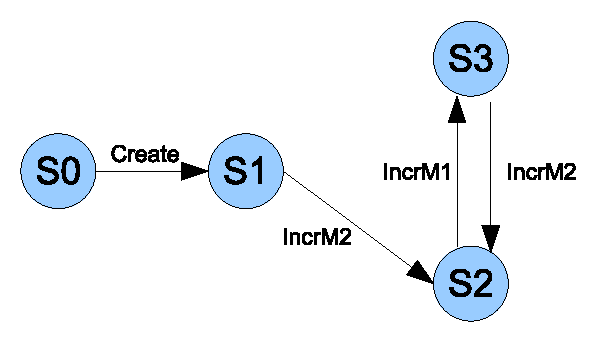
\includegraphics[scale=0.60,clip]{figs/MultiMethodsLoopFsa1.eps}
%\caption{\label{fig:loopfsa}Finite automaton for MultiMethodsLoop class.}
%\end{figure}
%
%These specifications can be inferred either by applying mining approaches on existing code bases~\cite{thummalapenta09:mseqgen} or from the implementation of the class under test~\cite{whaley02:interface}. Inferring complete specifications for all methods of the class under test can itself be a challenging problem that need to be addressed. For example, the approaches that infer specifications from the implementation are not scalable in practice. On the other hand, the approaches that infer specifications using mining approaches may not be able to infer specification for a method if that method is not used by any existing code bases. Therefore, a synergy of these two approaches can help effectively infer specifications.
%
%\subsection{Using specification for sequence generation}
%
%Our approach will next generate sequences that achieve desirable object states based on the inferred specification and the methods of interest. As we already know the methods of interest, the automaton representing can be pruned by not covering those paths that do not include our methods of interest. Next, our approach will explore this automaton to achieve the desired object state by visiting each method as desired number of times.
%
%\subsection{Open Problems}
%
%The current design is based on an assumption that it is possible to infer method summaries, which describe how methods of a class under test are modifying its fields. However, in case of classes from external libraries, it may not be possible to infer method summaries. 
\section{Preliminary Evaluation}
\label{sec:prelims}

We next present the preliminary results gathered by minually using the information from our approach. We use examples
from four real-world applications to show the preliminary results of our feasibility study. Column ``Before'' shows the block coverage achieved by Pex without the assistance from our approach. Column ``After'' shows the block coverage achieved after the assistance from the approach. The results show that Pex achieves better code coverages with the assistance of our approach.




\bibliographystyle{abbrv}
\bibliography{Seqex}

\end{document}
